\chapter{序論}\label{abst}
\section{背景と目的}

情報社会の発展に伴い, セキュリティシステムを利用する機会が増加している. 実世界, インターネットを含め, 最も多く利用されているのはパスワードに代表される知識ベースやICカード等を用いる物体ベースのシステム群である. これらは導入が容易ではあるが, 忘却や窃盗, 又は偽造(成りすまし)の問題が存在する\cite{cite_1}.

そこで現在, 盛んな研究と実用化が進められているのがバイオメトリクス認証技術である. こちらは認証のための情報として利用者の生体情報を使用する. 個人に固有の情報を用いるため, 他人による偽造が困難であること, 忘却や窃盗の心配が少ないことから, 従来よりも強固なセキュリティシステムの構築が期待される. 実用化されているバイオメトリクス認証システムでは主に指紋や静脈, 顔, 虹彩を認証情報として利用する\cite{cite_1}. これらはバイオメトリクスの中でも身体的特徴と呼ばれ, 本人と他人の弁別性が特に高い情報である. 非常に高精度な認証が可能であるが, これらの情報は本人であってもパスワードのように自由な変更が不可能である. そのため, もし一度でも他人に偽造された場合は一生涯に渡ってその情報の利用が不可能となる. また, 身体の情報をシステム側に提供することに抵抗を感じる人も存在する等, バイオメトリクス認証技術にも問題は存在する.

そこで, 本研究ではバイオメトリクス認証の手法として空中署名に注目した. これは, 空中に署名を行う動作からその人の癖や特徴を読み取り認証を行うもので, バイオメトリクスの中では行動的特徴に分類される. 本研究では署名を紙面上ではなく空中で行うため, 偽造は困難であるといえるが, 仮に他人に偽造されたとしても署名する文字は自由に変更可能である. そして, 身体の情報を直接使用しないため, 利用者も抵抗を感じにくいと考えられる. また, 署名による認証は署名文字と動作に含まれる癖の両方を用いる. 署名動作には一定の個人性・普遍性が含まれるが, それ単体では個人の特定は難しい. その意味で, 署名動作はソフトバイオメトリクスの側面も持つといえる. これは本研究成果の応用可能性として, その他ソフトバイオメトリクス情報との組み合わせにより, マルチモーダルソフトバイオメトリクス認証システムの構築も期待できることを示唆している.

以上より, 空中署名にはバイオメトリクスとして優れた性質があると考えられる. よって本研究では空中署名による個人認証を目指すこととする.


本文を書いていく.引用するときはciteを使う\cite{cite_1}.
citeの文字列はdocument.txtの参考文献の文字列と合わせる.
すると自動的に番号を振ってくれる.

段落分けする場合はこのように空行を挟む.

画像を張る場合は以下のように記述する.

\begin{figure}[htbp]
  \begin{center}
    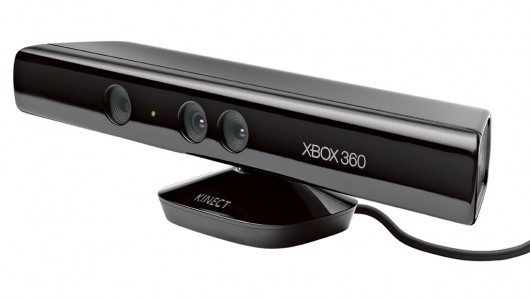
\includegraphics[clip,width=7.0cm]{./images/Kinect.jpg}
    \caption{Kinect}
    \label{fig:Kinect}
  \end{center}
\end{figure}

図ooと文中で用いる場合はrefを使用する図\ref{fig:Kinect}.
図のlabelとrefの文字列を合わせることで自動的に番号を振ってくれる.
includegraphicsの./images/ファイル名を変更することで表示する画像を変更できる.
使用できる画像は[.jpg .png .eps]のみ.

\section{論文構成}
本論文は全6章で構成される. 第1章では本研究における背景と目的を述べた. 第2章では署名による個人認証について, 第3章では関連研究を述べる. そして第4章で提案手法を, 第5章にて評価実験を述べた後, 第6章にて結論を述べる.
